Le Python est interprété, il nous faut donc un interpréteur! Il s'agit simplement d'un programme qui va lire notre code, et exécuter en temps réel les instructions qu'on lui donne.

Théoriquement, c'est le seul outil dont on a réellement besoin. Pratiquement, un développeur s'entoure d'une suite logicielle qui lui rend la vie bien plus facile. On utilisera énormément un \textit{éditeur de code}. C'est un éditeur de texte, à la manière de Microsoft Word, mais spécialisé dans un ou plusieurs langages de programmation. Il va notamment permettre de colorer le code pour le lire plus facilement, indenter automatiquement les lignes, les numéroter, etc.

\subsection{lancer un programme python}

On peut tout-à-fait utiliser l'éditeur de code et l'interpréteur séparément. Pour ce faire, il faut d'abord créer un fichier texte.\\
par exemple, ajoutons un nouveau fichier \textit{helloworld.txt} sur le bureau, qui contient exactement:
\begin{python}
print("Hello world !")
\end{python}
(notez que contrairement à Windows, l'extension .txt n'est pas nécéssaire à Raspbian, le système d'exploitation utilisé ici sur les raspberry pi.)
\\
Voilà notre premier programme en Python! Il sera expliqué par la suite, mais d'abord, lançons-le avec une invite de commande, aussi nommée le terminal. il se trouve dans la liste des programmes installés, ou en cliquant directement sur son icone noir dans la barre des tâches, ou encore avec le raccourci clavier $Ctrl + Alt + t$, mais le plus simple est de l'ouvrir via un click-droit sur le bureau->ouvrir en ligne de commande.

\subsection{Installer Spyder}

Les instructions suivantes permettent d'installer l'IDE \textit{Spyder}.

\begin{enumerate}
    \item Se rendre sur \url{https://www.continuum.io/downloads}.
    \item Télécharger l'installateur et suivre les instructions d'installation de celui-ci.
    \item Une fois l'installation terminée, lancer le programme \textit{Anaconda Navigator}.
    \item Depuis l'écran qui apparaît, lancer \textit{Spyder}.
\end{enumerate}

\subsection{Présentation de l'interface}

\begin{figure}[h!]
\begin{center}
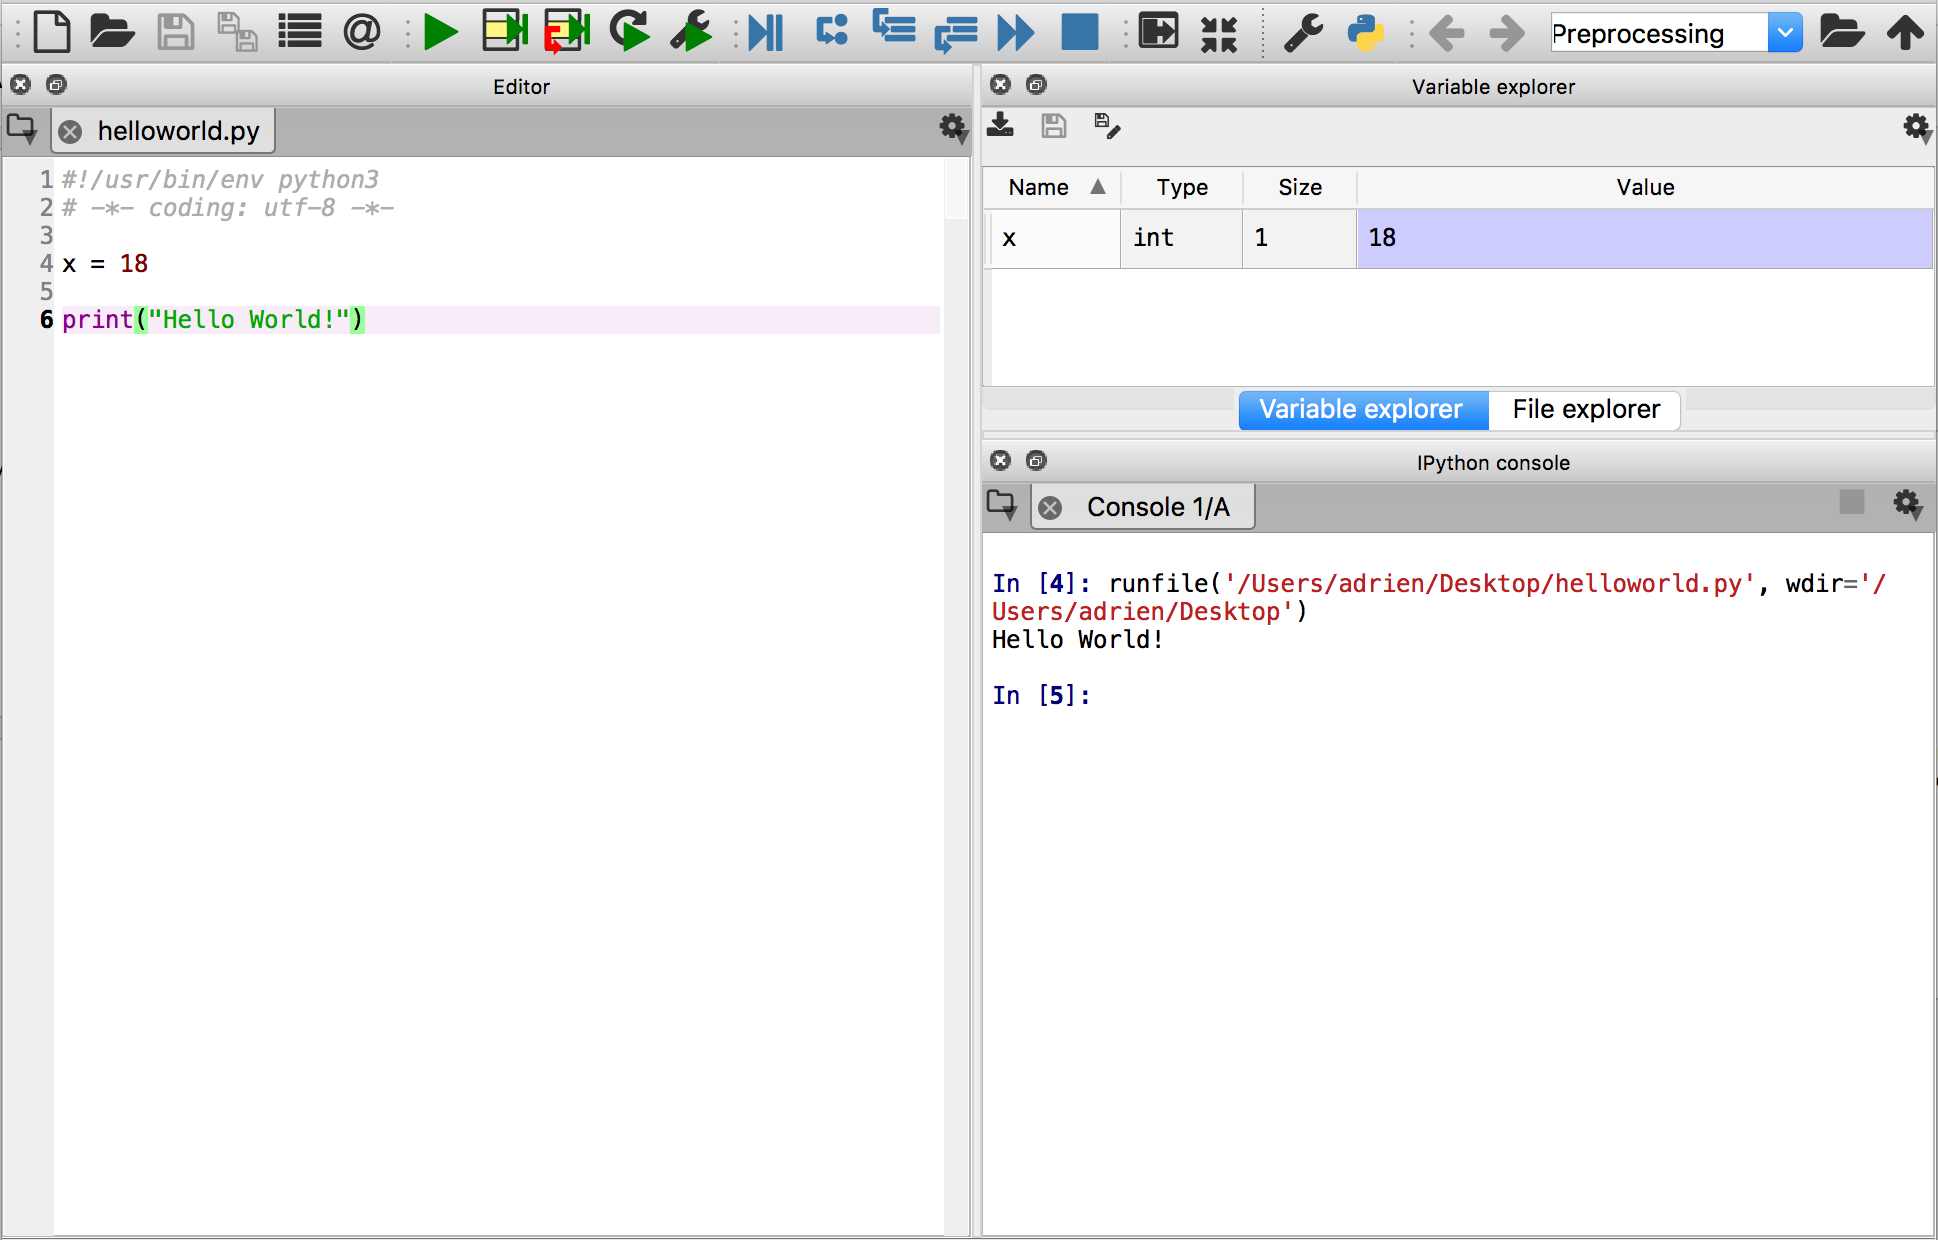
\includegraphics[width=15cm]{img/spyder.png}
\end{center}
\caption{Interface de Spyder}
\label{spyder}
\end{figure}

L'interface est simple à prendre en main. On retrouve 3 panneaux que nous utiliserons.
\begin{enumerate}
    \item A gauche, l'éditeur de code. C'est ici que nous écrirons le code source.
    \item En haut à droite, l'explorateur de variables. Probablement plus utile au début de l'apprentissage, on peut y voir les variables déclarées, et leur type.
    \item En bas à droit, la console. C'est ici que s'afficheront les résultats de nos programmes. On peut aussi directement y taper du code.
\end{enumerate}

Tout en haut, on trouve la barre d'outils. Les trois boutons de gauche servent respectivement à créer un fichier, ouvrir un fichier, et sauver le fichier. Enfin, la flèche verte permet d'exécuter le programme. Concrètement, l'interpréteur Python sera lancé, il lira le contenu de l'éditeur de code, et affichera le résultat dans la console.